\documentclass{beamer}
\usetheme[nomail]{Amurmaple}

\usepackage{amsfonts,amsmath,amssymb,amsthm}
\usepackage{xcolor}
\usepackage{graphicx,wrapfig}
\usepackage{booktabs}
\usepackage{tikz,pgfplots}
\usetikzlibrary{positioning}

\newtheorem{assum}{Assumption}

% Custom Commands
\newcommand{\argmax}{\arg\,\max}
\newcommand{\argmin}{\arg\,\min}
\newcommand{\bb}[1]{\mathbf{#1}}
\newcommand{\Mcal}{\mathcal{M}}
\newcommand{\Wcal}{\mathcal{W}}
\newcommand{\Pcal}{\mathcal{P}}
\newcommand{\E}{\mathbb{E}}
\newcommand{\var}{\text{Var}}
\newcommand{\prob}{\mathbb{P}}




%%%%%%%%
% Title and other metadata
\title[WISER]{\LARGE{Localized Detection of Authenticity in Mixed Source Texts via Epidemic Change-point Perspective}}
\author[S.~Roy]{Subhrajyoty Roy} 
\institute[WashU SDS]{Postdoctoral Researcher\\
Department of Statistics and Data Science\\ 
Washington University at St. Louis} 
\date{Oct 10, 2025} 
\titlegraphic{\includegraphics[width=4cm]{figures/logo.png}} 
\mail{roy.s@wustl.edu} 
% \webpage{www.ceremade.dauphine.fr/~chupin/}


\begin{document}

\maketitle

\begin{frame}{Collaborators}
    \begin{itemize}
        \item \alert{Soham Bonnerjee}, Department of Statistics, University of Chicago.
        \item \alert{Sayar Karmakar}, Department of Statistics, University of Florida.
    \end{itemize}
\end{frame}


\begin{frame}{Exponential Growth of LLM}
    \includegraphics[width=0.95\linewidth]{figures/llm-expo-graph.png}

    {\small\textbf{Latest Count from June, 2025:} $\approx 1.86M$.}
\end{frame}


\begin{frame}{Rise of LLM Generated Content}
    \includegraphics[width=0.8\linewidth]{figures/epium-content-generation.png}
    \includegraphics[width=0.6\linewidth]{figures/opeds_genai_declaration.png}
    \includegraphics[width=0.38\linewidth]{figures/nature article.png}
\end{frame}

\begin{frame}{Why we need authenticity verification?}
    \begin{itemize}
        \item \alert{Attribution:} Who wrote this? Human or AI?
        \item Academic Integrity.
        \item Misinformation (spam, political content).
        \item Intellectual Property / Copyrighting.
    \end{itemize}
\end{frame}

\begin{frame}{Emerging Issues with Academic Integrity}
    \includegraphics[width=\linewidth]{figures/emerging-academic-integrity.png}
\end{frame}

\begin{frame}{More Upcoming Threats!}
    \begin{enumerate}
        \item In order to train next generation of models, we need new datasets.
        \item Datasets are curated from the internet, which already contains AI generated texts.
        \pause
        \item Can create vicious loop, decreasing fairness, increasing ``not-so-good'' qualities.
    \end{enumerate}

    
    \begin{center}        
        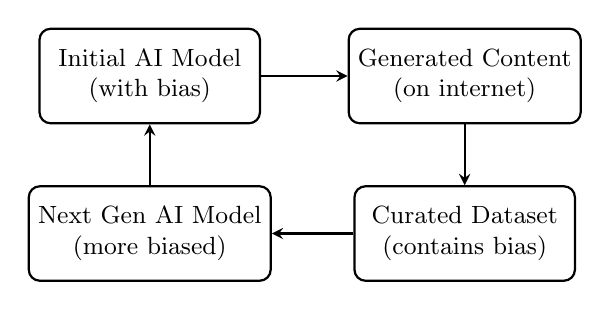
\begin{tikzpicture}[
            node distance=3cm,
            every node/.style={draw, rounded corners, align=center, minimum width=2.8cm, minimum height=1.2cm, font=\small},
            ->, >=stealth, thick
        ]

        % Nodes
        \node (ai1) {Initial AI Model \\ (with bias)};
        \node (gen) [right of=ai1, xshift=1cm] {Generated Content\\(on internet)};
        \node (data) [below of=gen, yshift = 1cm] {Curated Dataset \\ (contains bias)};
        \node (ai2) [left of=data, xshift = -1cm] {Next Gen AI Model \\ (more biased)};

        % Arrows
        \draw (ai1) -- (gen);
        \draw (gen) -- (data);
        \draw (data) -- (ai2);
        \draw (ai2) -- (ai1);
        \end{tikzpicture}
    \end{center}
\end{frame}

\begin{frame}
    Large-language models are trained to produce texts \alert{indistinguishable} from human-generated texts.\\
    \textcolor{red}{It is impossible to detect AI-generated vs human-generated content based on text alone.}

    \begin{center}
    \includegraphics[width=0.5\linewidth]{figures/hopeless-meme.jpg}        
    \end{center}

    \pause
    \alert{\textbf{Key Idea:}} Inject statistical signals (watermark) into AI-generated text that can be detected later! And here, statistics can help us!!
\end{frame}

\begin{frame}{The growth of ``explore''}
    % https://arxiv.org/pdf/2504.08755
    \begin{figure}[h]
    \includegraphics[width = 0.8\linewidth]{figures/explore word frequency.png}
    \caption[Monthly frequency of webpages]{Monthly frequency of webpages that contain the word ``explore''\footnote{\tiny Spennemann D. HR., ``Delving into'' the quantification of Ai-generated content on the internet, \url{https://arxiv.org/pdf/2504.08755}}}
    \end{figure}
\end{frame}

\begin{frame}{The growth of ``delve into''}
    % https://arxiv.org/pdf/2504.08755
    \begin{figure}[h]
    \includegraphics[width = 0.8\linewidth]{figures/delve-into-graph.png}
    \caption[Monthly frequency of webpages]{Monthly frequency of webpages that contain the word ``delve into''\footnote{\tiny Spennemann D. HR., ``Delving into'' the quantification of Ai-generated content on the internet, \url{https://arxiv.org/pdf/2504.08755}}}
    \end{figure}
\end{frame}

\begin{frame}{The Mechanism of Large Language Models}
    
   \only<1>{\begin{quotation}
       A large language model is an autocompletion system on streoids.
   \end{quotation}}

    \begin{center}
    \begin{tikzpicture}[node distance=1.5cm, >=stealth, font=\small]

    % Input tokens
    \only<2->{
        \node[draw, rounded corners, minimum width=1cm, minimum height=0.8cm] (w1) {Hi};

        \node[draw, thick, rounded corners, below=1.2cm of w1, minimum width=4.5cm, minimum height=1cm, fill=blue!10] (llm) {LLM};
        
        \draw[->] (w1.south) -- (llm.north);       
    }
    \only<2>{
        \node[draw, rounded corners, below=1.2cm of llm, minimum width=1cm, minimum height=0.8cm, fill=green!10] (o1) {How};
        \draw[->] (llm.south) -- (o1.north);
    }
    \only<3->{
        \node[draw, rounded corners, right=0.4cm of w1, minimum width=1cm, minimum height=0.8cm] (w2) {How};
        \draw[->] (w2.south) -- (llm.north); 
    }
    \only<3>{
        \node[draw, rounded corners, below=1.2cm of llm, minimum width=1cm, minimum height=0.8cm, fill=green!10] (o1) {are};
        \draw[->] (llm.south) -- (o1.north);
    }
    \only<4->{
        \node[draw, rounded corners, right=0.2cm of w2, minimum width=1cm, minimum height=0.8cm] (w3) {are};
        \draw[->] (w3.south) -- (llm.north); 
    }
    \only<4>{
        \node[draw, rounded corners, below=1.2cm of llm, minimum width=1cm, minimum height=0.8cm, fill=green!10] (o1) {you};
        \draw[->] (llm.south) -- (o1.north);
    }
    \only<5->{
        \node[draw, rounded corners, right=0.4cm of w3, minimum width=1cm, minimum height=0.8cm] (w4) {you};
        \draw[->] (w4.south) -- (llm.north); 
    }
    \only<5>{
        \node[draw, rounded corners, below=1.2cm of llm, minimum width=1cm, minimum height=0.8cm, fill=green!10] (o1) {?};
        \draw[->] (llm.south) -- (o1.north);
    }
    \only<6->{
        \node[draw, rounded corners, right=0.4cm of w4, minimum width=1cm, minimum height=0.8cm] (w5) {?};
        \draw[->] (w5.south) -- (llm.north); 
    }
    \only<6>{
        \node[draw, rounded corners, below=1.2cm of llm, minimum width=1cm, minimum height=0.8cm, fill=green!10] (o1) {$\langle EOS\rangle$};
        \draw[->] (llm.south) -- (o1.north);
    }

    \end{tikzpicture}
    \end{center}

    \only<6>{Given $w_1, w_2, \dots, w_{t-1}$, the LLM $\Mcal$ outputs a next token probability distribution $P_t$ over the vocabulary $\Wcal$. The next token is chosen as $w_t \sim P_t$.}
\end{frame}


\begin{frame}{Red Green Watermark}

    \begin{enumerate}
        \item Assign words in the vocabulary $\Wcal$ to either \textcolor{red}{Red} $R$ or \textcolor{green}{Green} $G$ bucket.
        \item After LLM produces $P_t$, compute logits from $P_t$, say $l_t(w)$ for each $w \in \Wcal$.
        \item Define,
        \begin{equation*}
            P_t^{(rg)}(w) = \dfrac{\exp(l_t(w) + \delta \bb{1}(w \in G) )}{\sum_{w \in \Wcal} \exp(l_t(w) + \delta \bb{1}(w \in G) )}
        \end{equation*}
        \item Sample $w_t \sim P^{(rg)}_t$.
    \end{enumerate}
\end{frame}

\begin{frame}{Red Green Watermark (Contd.)}
    \includegraphics[width = \linewidth]{figures/red-green-watermark.png}

    \pause

    \begin{alertblock}{Detection Rule}
        Let $\vert G \vert = \gamma \vert \Wcal\vert$. There is a presence of watermark if 
        \begin{equation*}
            \dfrac{\frac{1}{T}\text{(\# of tokens from } G)  - \gamma}{\sqrt{\frac{\gamma (1 - \gamma)}{T}}} \text{ is large}
        \end{equation*}
    \end{alertblock}

    \pause 
    \textcolor{red}{\textbf{Problem:}} It modifies the token distribution $P_t$ to something else.
\end{frame}

\begin{frame}{Gumbel-max Trick\footnote{\tiny Aaronson, 2023. \url{https://www.youtube.com/watch?v=2Kx9jbSMZqA}}}
    \begin{enumerate}
        \item Use LLM $\Mcal$ to produce NTP $P_t$.
        \item Generate i.i.d. random variables $U_1, U_2, \dots, U_{\vert \Wcal\vert} \sim U(0, 1)$.
        \item Output 
        \begin{equation*}
            w_t = \argmax_{w \in \Wcal} \frac{\log(U_w)}{P_t(w)}
        \end{equation*}
        \item Turns out, $w_t$ still follows $P_t$.
        \item But we know that if $w_t$ is selected, that means $\log(U_{w_t})$ must be large, or $U_{w_t} \approx 1$.
    \end{enumerate}
\end{frame}

\begin{frame}{General Framework for LLM Watermark}
    \begin{enumerate}
        \item Based on $w_1, \dots, w_{t-1}$, use LLM to generate $P_t$.
        \item Based on $w_1, \dots, w_{t-1}$, generate a pseudorandom seed $\xi_t := \text{Hash}(w_1, \dots, w_{t-1}; \text{Key})$.
        \item Use a decoding strategy $w_t \leftarrow S(P_t, \xi_t)$.
        \pause
        \item If $w_t$ is human-generated, we don't expect $w_t$ to be correlated with $\xi_t$ in any way.
        \pause
        \item If $w_t$ is AI-generated, the decoder $S(\cdot)$ creates some dependency between $w_t$ and $\xi_t$.
        \pause
        \item There is a \alert{pivot statistic} $Y_t = h(w_t, \xi_t)$ which tracks this dependency; it is large if $w_t$ is correlated with $\xi_t$.
    \end{enumerate}
\end{frame}

\begin{frame}{Example}
    \begin{figure}[h]
        \centering
        \includegraphics[width=\linewidth]{figures/text_example.jpeg}
        \includegraphics[width=\linewidth]{figures/wm_diagram_pivot.png}
        \caption{[Top]: Example Sentence where tokens $70-100$ has been watermarked. [Bottom]: Corresponding pivot statistic.}
    \end{figure}
\end{frame}

\begin{frame}{Hypothesis Testing Framework}
    \begin{align*}
        H_0: & {} w_t \text{ is unwatermarked}\\
        H_1: & {} w_t \text{ is watermarked}
    \end{align*}

    \begin{lemma}
        Under $H_0$, $Y_t := S(w_t, \xi_t)$ are i.i.d. with mean say $\E(Y_t) = \mu_0$
    \end{lemma}

    \begin{alertblock}{Assumption}
        Under $H_1$, say $P_t \in \Pcal$, then 
        \begin{equation*}
            \inf_{P \in \Pcal} \E_{1}(Y_t) \geq \mu_0 + d
        \end{equation*}
        \noindent for some constant $d > 0$.
    \end{alertblock}
\end{frame}

\begin{frame}{Existing Literature}
    % TODO: discuss some existing types of works

    \begin{itemize}
        \item Detection of presence of watermark in single-source texts\footnote{\tiny Li et al (2025) - A statistical framework of watermarks for large language models: Pivot, detection efficiency and optimal rules}. Can be formalized via hypothesis testing framework, and solved via likelihood ratio test.
        \pause
        \item Estimation of the proportion of AI-generated content in mixed-source texts\footnote{\tiny Li et al (2025) - Optimal estimation of watermark proportions in hybrid ai-human texts}. Formalized using Huber's contamination model 
        \begin{equation*}
            P_{obs,t}(w) = (1-\epsilon)P_t(w) + \epsilon P_{\text{watermarked}, t}(w),
        \end{equation*}
        \noindent and $\epsilon$ is estimated using weighted-moment method.
        \pause
        \item Much less work on estimating segments / patches of watermarked text\footnote{\tiny Pan et al. (2025) - Waterseeker: Pioneering efficient detection of watermarked segments in large documents}. Typically slow, requires $O(n\log(n))$ time.
    \end{itemize}
\end{frame}


\begin{frame}{Epidemic Changepoint}
    \begin{itemize}
        \item In epidemiology, \textcolor{blue}{Levin and Klein (1985)}\footnote{\tiny``The cusum test of homogeneity with an application in spontaneous abortion epidemiology.'' - Levin and Klein, 1985.}, first studied this kind of changepoint problem, where the changes occur in a segment of time.
        \item \alert{Epidemic} changepoint helps to track when an epidemic starts and ends. If reproduction number of virus ($R$) exceeds $1$, epidemic starts, if it is below $1$, epidemic ends.
        \pause
        \item This is different from the standard changepoint problem.
        \begin{itemize}
            \item The estimated changepoints must occur in pairs.
            \item Estimation of ``no'' changepoint, may correspond to either \alert{the entire text is watermarked} or \alert{the entire text is unwatermarked}.
            \item When the text is unwatermarked, then the distribution of pivot statistic is \alert{completly known}.
        \end{itemize}
    \end{itemize}
\end{frame}


\begin{frame}{WISER: Watermark Identification via Segmenting Epidemic Region}

\begin{columns}[T]
    \begin{column}{0.5\textwidth}
        \begin{enumerate}
        \item<1-> Given $\{Y_t\}_{t=1}^n$, create blocks of length $b \approx \sqrt{n}$. Calculate block sums $S_1, \dots, S_{[n/b]}$.
        \item<2-> Keep blocks where $S_i > \mathbb{Q}$, and $\mathbb{Q}$ is $(1-\alpha)$-th quantile of null distribution of maximum block sum.
        \end{enumerate}
    \end{column}
    \begin{column}{0.5\textwidth}
        \includegraphics[width = \linewidth]{figures/wiser-stage1.png}
    \end{column}
\end{columns}
    
\end{frame}

\begin{frame}{WISER: Watermark Identification via Segmenting Epidemic Region}
    
\begin{columns}[T]
    \begin{column}{0.5\textwidth}
        \begin{enumerate}
        \setcounter{enumi}{2}
        \item<1-> Join the selected consecutive blocks and discard blocks smaller than $c\sqrt{n}$.
        \item<2-> Slightly enlarge each block (by $cn^{\gamma}$ on both sides for small $\gamma \approx 0.1$), call them $D_i$.
        \end{enumerate}
    \end{column}
    \begin{column}{0.5\textwidth}
        \includegraphics[width = \linewidth]{figures/wiser-stage2.png}
    \end{column}
\end{columns}
\end{frame}


\begin{frame}{WISER: Watermark Identification via Segmenting Epidemic Region}
    
\begin{enumerate}
    \setcounter{enumi}{4}
    \item Estimate $d$ using average of $Y_t - \mu_0$ over detected blocks, i.e., over $\cup_{i=1}^{\hat{K}} D_i$.
    \item Locally adjust each detected block interval $D_i = (L_i, R_i)$ (let $M_i = (L_i + R_i)/2$) using:
    \begin{equation*}
        \hat{I}_i := \text{argmin}_{l \in (L_i, M_i), r \in (M_{i}+1, R_i)} \sum_{t \notin D_j \setminus (l, r)} (Y_t - \mu_0 - \rho \hat{d})
    \end{equation*}
\end{enumerate}

\end{frame}



\begin{frame}{Assumptions}
    \textbf{Assumption 1:} Each true watermarked interval $\{ I_j \}_{j=1}^K$ have size $O(\sqrt{n})$.\\

    \medskip
    \alert{Ensures that the first stage with block size $\sqrt{n}$ has enough signal to detect.}\\

    \medskip
    
    \pause
    \textbf{Assumption 2:} Any two consecutive intervals have gaps at least $O(\sqrt{n})$.\\
    \medskip

    % TODO: Give image
    \alert{Consecutive detected intervals may end up joining into single interval.}\\

\end{frame}

\begin{frame}{Assumptions (Contd.)}
    \textbf{Assumption 3:} $\min\{ \var_0(Y_t), \sup_{P \in \Pcal} \var_{1}(Y_t) \} > 0$.\\
    \medskip

    % TODO Show the example of asking factual question
    \begin{center}
        \includegraphics[width=\linewidth]{figures/chatgpt-novar.png}
    \end{center}

    Prompts that have \alert{deterministic} completion will always remain same whether watermarked or NOT watermarked. 
\end{frame}




\begin{frame}{Theoretical Validation}
    \begin{theorem}[Simplified]
        Assume that:
        \begin{enumerate}
            \item Each true watermarked interval $\{ I_j \}_{j=1}^K$ have size $O(\sqrt{n})$
            \item Any two consecutive intervals have gaps at least $O(\sqrt{n})$.
            \item $\min\{ \var_0(Y_t), \sup_{P \in \Pcal} \var_{1}(Y_t) \} > 0$.
            \item $\sup_{P \in \Pcal} \E_{1,P}(\eta \vert Y_t\vert) < \infty$ for some $\eta > 0$.
        \end{enumerate}

        Then, as $n \to \infty$, 
        \begin{equation*}
            \prob\left( \hat{K} = K; \ \min_{1 \leq j \leq K} \vert I_j \Delta \hat{I}_j\vert < \frac{M}{d} \right) \to 1
        \end{equation*}
    \end{theorem}
\end{frame}

\begin{frame}{Results}
    \includegraphics[width = \textwidth]{figures/wiser-output.png}
\end{frame}

\begin{frame}{Benchmark Results (Gumbel)}
    \begin{center}
        \includegraphics[width=\linewidth]{figures/gumbel-result.png}
    \end{center}
\end{frame}

\begin{frame}{Benchmark Results (Red-Green)}
    \begin{center}
        \includegraphics[width=\linewidth]{figures/redgreen-result.png}
    \end{center}    
\end{frame}

\begin{frame}{Time Complexity}
    \begin{center}
        \includegraphics[width=\linewidth]{figures/time-complexity.png}\\
        Time complexity of \texttt{WISER} is $O(K n)$.
    \end{center}
\end{frame}

\begin{frame}{Effect of Block Size}
    \begin{center}
        \includegraphics[width=\linewidth]{figures/ablation_block_size.png}\\
        Here, $n \approx 500$, so a block size of $\sqrt{n} \approx 22$ is appropriate.
    \end{center}    
\end{frame}

\begin{frame}{Summarization}
    \begin{itemize}
        \item Watermarking is way to inject statistical signals into LLM-generated text, so that authenticity can be established.
        \item Various watermarking schemes exist, some are biased, some are unbiased.
        \item \texttt{WISER}\footnote{\tiny\url{https://www.github.com/subroy13/wiser}} can be used to efficiently detect watermarked regions in mixed-source texts. It is fast, theoretically valid, and works across multiple models and multiple watermarking schemes.
    \end{itemize}
\end{frame}


\begin{frame}{There are still things to do!}
    % Talk about Paraphrasing and Emoji attacks (limitations)
    \begin{center}
        \includegraphics[width=0.8\textwidth]{figures/emoji-attack.png}\\

        Other attacks include \alert{letter-switching, translation,} etc.
    \end{center}    
\end{frame}



\thanksframe{Thank you!}


\end{document}